\section{From Classical Prediction to Learned Representations}

Chapter 1 ended with a structural observation that now becomes the starting point of this chapter. Many learning systems can be written in compositional form:
\[
f = g\circ \phi.
\]
The decisive question is therefore not only which predictor $g$ should be fit, but also whether the representation map $\phi$ is fixed in advance or learned from data.

This section makes that contrast concrete by following a classical path:
\begin{center}
perceptron $\to$ logistic regression $\to$ regularization $\to$ margin $\to$ SVM $\to$ kernels $\to$ limits of fixed representations $\to$ neural networks.
\end{center}
The goal is not to turn the chapter into a full course on support vector machines, but to show why large-margin methods are the high point of the classical fixed-feature pipeline and why deep learning becomes attractive when useful representations are not available in advance.

\subsection*{A formal decomposition of classical prediction}

Let $\mathcal X$ be the input space, $\mathcal Z$ a feature space, and $\mathcal Y$ the output space. A representation map
\[
\phi:\mathcal X\to\mathcal Z
\]
transforms raw inputs into features, while a predictor
\[
g:\mathcal Z\to\mathcal Y
\]
acts on those features.

\begin{definition}[Fixed-feature predictive pipeline]
A \emph{fixed-feature predictive pipeline} is a predictor of the form
\[
f = g\circ \phi,
\]
where the representation map $\phi$ is specified in advance and only the predictor $g$ is learned from data.
\end{definition}

This description covers a large fraction of classical machine learning. The features may be polynomial expansions, hand-crafted signal descriptors, bag-of-words vectors, random features, or kernel-induced coordinates. The learning algorithm then operates on those features rather than on the raw input directly.

\begin{proposition}[Fixed representations induce hypothesis classes]
Let $\phi:\mathcal X\to\mathcal Z$ be a fixed representation map, and let $\mathcal G$ be a class of predictors from $\mathcal Z$ to $\mathcal Y$. Then $\phi$ induces a hypothesis class on $\mathcal X$ given by
\[
\mathcal H_\phi=\{g\circ\phi : g\in\mathcal G\}.
\]
In contrast, when both the representation map and the predictor are learned, the effective hypothesis class takes the form
\[
\mathcal H=\{g\circ\phi : \phi\in\Phi,\ g\in\mathcal G\},
\]
which is generally much richer.
\end{proposition}

\begin{proof}
If $\phi$ is fixed, then every candidate predictor on $\mathcal X$ is obtained by composing $\phi$ with some $g\in\mathcal G$. Hence the available functions on the original input space are exactly
\[
\{g\circ\phi : g\in\mathcal G\}.
\]
If, on the other hand, the representation itself can vary over a family $\Phi$, then the learner may choose both a representation and a predictor, producing the larger composed class
\[
\{g\circ\phi : \phi\in\Phi,\ g\in\mathcal G\}.
\]
\end{proof}

This proposition is simple but fundamental. It makes clear that feature design is not a cosmetic preprocessing step. It directly determines the hypothesis class the learner can realize.

\subsection*{The classical path: from separability to margin}

The perceptron and logistic regression are natural starting points because both use an affine score
\[
s(x)=w^\top \phi(x)+b,
\]
but interpret and train that score differently.

\paragraph{Perceptron.}
The perceptron predicts by thresholding the sign of the score. Its geometry is crisp: it asks whether a hyperplane can separate the two classes.

\paragraph{Logistic regression.}
Logistic regression uses the same affine score but passes it through a sigmoid or softmax and optimizes a smooth likelihood-based loss. The output is naturally interpreted in probabilistic terms.

\paragraph{Regularization.}
As Chapter 1 already emphasized, fitting the training data is not the whole story. A penalty such as $\lambda\|w\|^2$ controls the scale of the classifier and influences which separator is preferred among many that fit the sample.

These three ideas lead directly to the margin viewpoint. If many separators classify the data correctly, it is natural to ask whether some are geometrically better than others.

\begin{figure}[tbp]
\centering
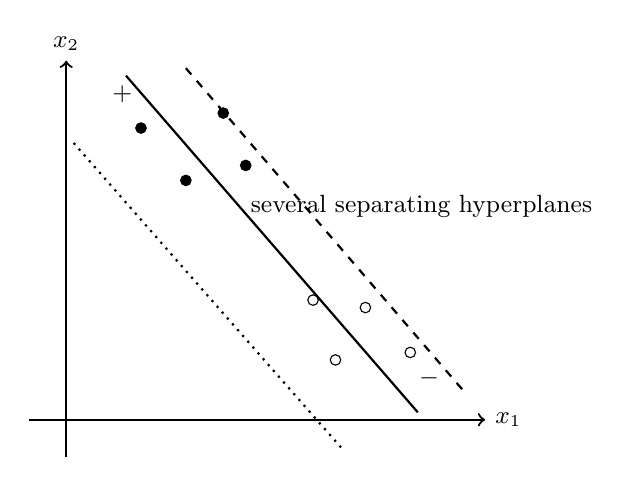
\begin{tikzpicture}[scale=0.95,
    axis/.style={->, thick},
    sep/.style={thick},
    every node/.style={font=\small}
]
    \draw[axis] (-0.5,0) -- (5.6,0) node[right] {$x_1$};
    \draw[axis] (0,-0.5) -- (0,4.8) node[above] {$x_2$};

    % positives
    \filldraw (1.0,3.9) circle (2pt);
    \filldraw (1.6,3.2) circle (2pt);
    \filldraw (2.1,4.1) circle (2pt);
    \filldraw (2.4,3.4) circle (2pt);
    % negatives
    \filldraw[fill=white] (3.6,0.8) circle (2pt);
    \filldraw[fill=white] (4.0,1.5) circle (2pt);
    \filldraw[fill=white] (4.6,0.9) circle (2pt);
    \filldraw[fill=white] (3.3,1.6) circle (2pt);

    % hyperplanes
    \draw[sep] (0.8,4.6) -- (4.7,0.1);
    \draw[sep,dashed] (1.6,4.7) -- (5.3,0.4);
    \draw[sep,dotted] (0.1,3.7) -- (3.7,-0.4);

    \node at (4.75,2.85) {several separating hyperplanes};
    \node at (0.75,4.35) {$+$};
    \node at (4.85,0.55) {$-$};
\end{tikzpicture}
\caption{Linearly separable data can admit many separating hyperplanes. Margin-based methods ask not only for separation, but for a separator that stays as far as possible from the closest training points.}
\end{figure}

\subsection*{Why margin matters}

Suppose binary labels satisfy $y_i\in\{-1,1\}$ and the classifier is
\[
f(x)=\operatorname{sign}(w^\top x+b).
\]
A point is correctly classified when $y_i(w^\top x_i+b)>0$. But correct classification alone does not distinguish a fragile separator from a robust one.

\begin{definition}[Functional margin]
For a labeled example $(x_i,y_i)$ and affine score $s(x)=w^\top x+b$, the \emph{functional margin} is
\[
y_i(w^\top x_i+b).
\]
For a dataset, the functional margin is the minimum of this quantity over all training examples.
\end{definition}

The functional margin depends on scale. If we multiply $(w,b)$ by a positive constant, the classifier does not change, but the functional margin does. The geometric margin corrects for this.

\begin{definition}[Geometric margin]
The \emph{geometric margin} of $(x_i,y_i)$ with respect to $(w,b)$ is
\[
\frac{y_i(w^\top x_i+b)}{\|w\|}.
\]
For a dataset, the geometric margin is the minimum of this quantity over the sample.
\end{definition}

\begin{proposition}[Margin is scale-invariant after normalization]
For any $c>0$, the classifiers $(w,b)$ and $(cw,cb)$ define the same decision boundary. Their functional margins differ by a factor of $c$, but their geometric margins are equal.
\end{proposition}

\begin{proof}
The sign of $cw^\top x+cb$ is the same as the sign of $w^\top x+b$ for every $x$ because $c>0$. Thus the decision boundary is unchanged. The functional margin becomes
\[
y_i(cw^\top x_i+cb)=c\,y_i(w^\top x_i+b),
\]
so it scales by $c$. The geometric margin becomes
\[
\frac{y_i(cw^\top x_i+cb)}{\|cw\|}
=
\frac{c\,y_i(w^\top x_i+b)}{c\|w\|}
=
\frac{y_i(w^\top x_i+b)}{\|w\|},
\]
which is unchanged.
\end{proof}

This is why the geometric margin is the meaningful object. It measures distance to the decision boundary rather than arbitrary parameter scale.

\subsection*{Hard-margin SVM}

If the data are linearly separable, one can ask for the separator of largest geometric margin. By scaling $(w,b)$ so that the closest points satisfy
\[
y_i(w^\top x_i+b)\ge 1,
\]
maximizing geometric margin becomes equivalent to minimizing $\|w\|$.

\begin{definition}[Hard-margin support vector machine]
For linearly separable data, the \emph{hard-margin SVM} solves
\[
\min_{w,b}\ \frac12\|w\|^2
\qquad
\text{subject to}
\qquad
y_i(w^\top x_i+b)\ge 1
\quad\text{for all }i.
\]
\end{definition}

\begin{figure}[tbp]
\centering
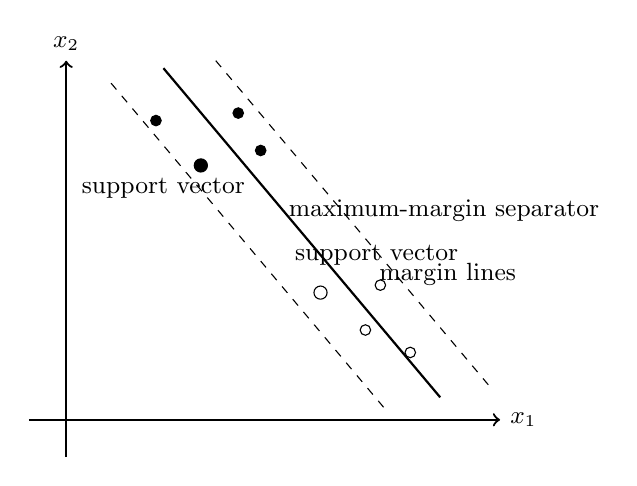
\begin{tikzpicture}[scale=0.95,
    axis/.style={->, thick},
    line main/.style={thick},
    line margin/.style={dashed},
    sv/.style={circle, draw, inner sep=1.2pt},
    every node/.style={font=\small}
]
    \draw[axis] (-0.5,0) -- (5.8,0) node[right] {$x_1$};
    \draw[axis] (0,-0.5) -- (0,4.8) node[above] {$x_2$};

    % main separator and margins
    \draw[line main] (1.3,4.7) -- (5.0,0.3);
    \draw[line margin] (0.6,4.5) -- (4.3,0.1);
    \draw[line margin] (2.0,4.8) -- (5.7,0.4);

    % points
    \filldraw (1.2,4.0) circle (2pt);
    \filldraw[sv] (1.8,3.4) circle (2.5pt);
    \filldraw (2.3,4.1) circle (2pt);
    \filldraw (2.6,3.6) circle (2pt);

    \filldraw[fill=white,sv] (3.4,1.7) circle (2.5pt);
    \filldraw[fill=white] (4.0,1.2) circle (2pt);
    \filldraw[fill=white] (4.6,0.9) circle (2pt);
    \filldraw[fill=white] (4.2,1.8) circle (2pt);

    \node at (1.3,3.1) {support vector};
    \node at (4.15,2.2) {support vector};
    \node at (5.05,2.8) {maximum-margin separator};
    \node at (5.1,1.95) {margin lines};
\end{tikzpicture}
\caption{Hard-margin geometry. The central line is the decision boundary, the dashed lines mark equal-distance margin boundaries, and the nearest points are the support vectors. Only those closest points determine the optimal separator.}
\end{figure}

The geometry now becomes very clean. A large-margin separator is not merely one that classifies correctly; it is one that keeps the boundary away from the closest training examples.

\subsection*{Soft margin, slack, and regularization}

Real data are rarely perfectly separable. Noise, overlap, or label ambiguity may force some violations. The soft-margin SVM introduces slack variables $\xi_i\ge 0$:
\[
y_i(w^\top x_i+b)\ge 1-\xi_i.
\]
The optimization problem becomes
\[
\min_{w,b,\xi}\ \frac12\|w\|^2 + C\sum_{i=1}^n \xi_i
\qquad
\text{subject to}
\qquad
\xi_i\ge 0,
\quad
y_i(w^\top x_i+b)\ge 1-\xi_i.
\]

The parameter $C$ trades off two goals:
\begin{itemize}
    \item keeping the separator simple and large-margin through $\|w\|^2$;
    \item penalizing violations through the slack terms.
\end{itemize}
This is regularization in action. The model does not merely search for any classifier with low training error; it balances data fit against separator scale.

\begin{figure}[tbp]
\centering
\begin{tikzpicture}[scale=0.95,
    axis/.style={->, thick},
    line main/.style={thick},
    line margin/.style={dashed},
    slack/.style={-{Latex[length=2mm]}, thick},
    every node/.style={font=\small}
]
    \draw[axis] (-0.5,0) -- (5.8,0) node[right] {$x_1$};
    \draw[axis] (0,-0.5) -- (0,4.8) node[above] {$x_2$};

    \draw[line main] (1.4,4.7) -- (5.1,0.2);
    \draw[line margin] (0.7,4.5) -- (4.4,0.0);
    \draw[line margin] (2.1,4.8) -- (5.8,0.3);

    \filldraw (1.0,4.0) circle (2pt);
    \filldraw (2.0,3.6) circle (2pt);
    \filldraw (2.4,4.2) circle (2pt);

    \filldraw[fill=white] (3.7,1.1) circle (2pt);
    \filldraw[fill=white] (4.2,1.6) circle (2pt);
    \filldraw[fill=white] (4.7,0.9) circle (2pt);

    % violating point
    \filldraw[fill=white] (3.05,2.15) circle (2.2pt);
    \draw[slack] (3.05,2.15) -- (3.52,1.58);
    \node at (2.45,2.55) {violating point};
    \node at (3.75,2.35) {slack};
\end{tikzpicture}
\caption{Soft-margin SVM allows some points to lie inside the margin or even on the wrong side of the boundary. Slack variables measure the size of these violations, and the objective penalizes them while still preferring a large-margin separator.}
\end{figure}

\subsection*{Why SVM is not just another linear classifier}

At first glance, perceptron, logistic regression, and a linear SVM all use the score $w^\top x+b$. But they embody different learning principles:
\begin{itemize}
    \item the perceptron focuses on correcting mistakes;
    \item logistic regression models class probabilities through a smooth loss;
    \item SVM focuses on the geometry of margin and the scale of the separator.
\end{itemize}

\commonconfusion{An SVM is not ``just another linear classifier.'' In a linear SVM, the decision boundary is linear in the chosen feature space, but the method is distinguished by the margin principle, the role of support vectors, and the explicit control of separator scale through regularization. With kernels, the boundary can also become highly nonlinear in the original input space even though the classifier remains linear in feature space.}

\subsection*{The kernel viewpoint}

A key classical insight is that linear prediction in a feature space can look nonlinear in the original coordinates. If one chooses a nonlinear map
\[
\phi(x),
\]
and then applies a linear classifier in the $\phi$-coordinates, the resulting boundary in input space can be curved and expressive.

The kernel trick pushes this idea further. Rather than write $\phi(x)$ explicitly, one works with inner products
\[
K(x,x') = \langle \phi(x),\phi(x')\rangle.
\]
The predictor can then be written in terms of similarities to selected training points.

\begin{figure}[tbp]
\centering
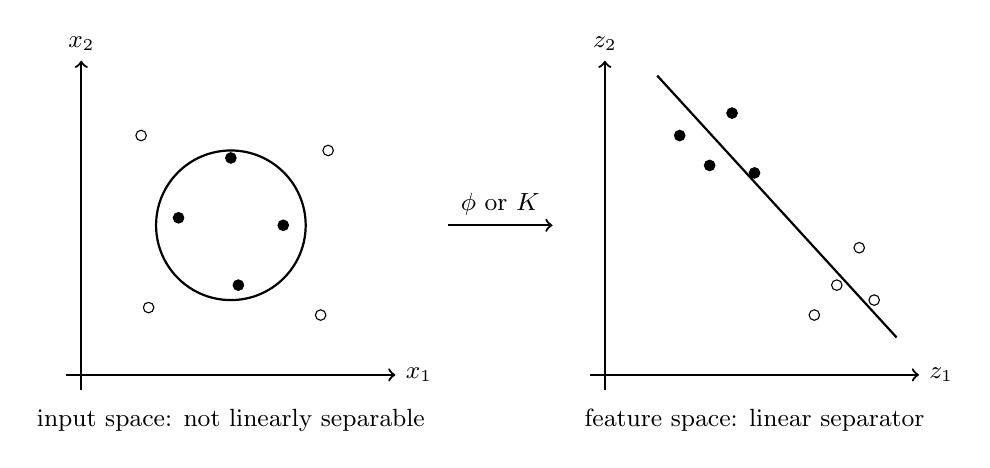
\begin{tikzpicture}[scale=0.95, every node/.style={font=\small}]
    % left panel: input space
    \begin{scope}
        \draw[->, thick] (-0.2,0) -- (4.2,0) node[right] {$x_1$};
        \draw[->, thick] (0,-0.2) -- (0,4.2) node[above] {$x_2$};
        \draw[thick] (2,2) circle (1.0);
        \filldraw (2.0,2.9) circle (2pt);
        \filldraw (2.7,2.0) circle (2pt);
        \filldraw (1.3,2.1) circle (2pt);
        \filldraw (2.1,1.2) circle (2pt);
        \filldraw[fill=white] (0.8,3.2) circle (2pt);
        \filldraw[fill=white] (3.3,3.0) circle (2pt);
        \filldraw[fill=white] (3.2,0.8) circle (2pt);
        \filldraw[fill=white] (0.9,0.9) circle (2pt);
        \node at (2,-0.6) {input space: not linearly separable};
    \end{scope}

    % arrow
    \draw[->, thick] (4.9,2.0) -- (6.3,2.0) node[midway, above] {$\phi$ or $K$};

    % right panel: feature space
    \begin{scope}[xshift=7.0cm]
        \draw[->, thick] (-0.2,0) -- (4.2,0) node[right] {$z_1$};
        \draw[->, thick] (0,-0.2) -- (0,4.2) node[above] {$z_2$};
        \filldraw (1.0,3.2) circle (2pt);
        \filldraw (1.4,2.8) circle (2pt);
        \filldraw (1.7,3.5) circle (2pt);
        \filldraw (2.0,2.7) circle (2pt);
        \filldraw[fill=white] (3.1,1.2) circle (2pt);
        \filldraw[fill=white] (3.4,1.7) circle (2pt);
        \filldraw[fill=white] (2.8,0.8) circle (2pt);
        \filldraw[fill=white] (3.6,1.0) circle (2pt);
        \draw[thick] (0.7,4.0) -- (3.9,0.5);
        \node at (2,-0.6) {feature space: linear separator};
    \end{scope}
\end{tikzpicture}
\caption{A toy nonlinear dataset and its kernelized viewpoint. In the original coordinates the classes may not be linearly separable, but after a suitable feature lifting, a linear separator can become available. Kernel methods realize this idea without always writing the feature map explicitly.}
\end{figure}

Kernels are therefore a powerful extension of the fixed-feature pipeline. They allow nonlinear decision boundaries while preserving the basic classical structure:
\begin{quote}
choose a representation geometry first, then fit a shallow predictor inside it.
\end{quote}

\subsection*{A comparative summary}

\begin{table}[tbp]
\centering
\renewcommand{\arraystretch}{1.25}
\begin{tabular}{p{2.5cm}p{2.6cm}p{3.0cm}p{2.5cm}p{2.2cm}}
\toprule
\textbf{Method} & \textbf{Representation} & \textbf{Learning principle} & \textbf{Typical output view} & \textbf{Main limitation} \\
\midrule
Perceptron
& raw inputs or fixed features
& update on mistakes for a separating hyperplane
& hard classification
& requires linear separability for its clean guarantee \\
\addlinespace
Logistic regression
& raw inputs or fixed features
& smooth likelihood / cross-entropy minimization
& probabilistic score
& still shallow unless features are enriched \\
\addlinespace
SVM
& fixed explicit or kernel features
& maximize margin while controlling scale
& large-margin classifier
& representation is still fixed in advance \\
\addlinespace
Neural network
& learned intermediate representations
& joint optimization of many composed maps
& flexible task-dependent predictor
& optimization and generalization are more complex \\
\bottomrule
\end{tabular}
\caption{A comparison that clarifies the conceptual transition. Perceptron, logistic regression, and SVM differ in training principle, but all remain shallow methods on a chosen representation. Neural networks change the game by learning the representation itself.}
\end{table}

\subsection*{The limit of fixed representations}

Classical methods can be extremely powerful when the right representation is available. A handcrafted signal descriptor, a good polynomial basis, or a well-chosen kernel may transform a hard problem into one that a shallow predictor solves elegantly.

But that strategy has a ceiling. If the task requires discovering many levels of abstraction from raw data---edges to parts to objects, phonemes to words to meanings, local patterns to global structure---then a fixed representation may be too rigid. The learner can only optimize within the geometry already chosen for it.

This is the key limitation of the classical pipeline. Its strength is clean geometry and often cleaner optimization. Its weakness is dependence on representation choices made before training begins.

\whattoremember{The classical fixed-feature pipeline can be summarized as $f=g\circ\phi$: choose a representation, then fit a shallow rule. Perceptron, logistic regression, and SVM all fit this picture, even when kernels make the induced boundary nonlinear in the original input space. Margin turns linear separation into a geometric optimization problem, and soft-margin SVM shows how regularization controls the tradeoff between separator scale and training violations. The decisive limitation is that the representation is fixed in advance. Neural networks will matter in the rest of the chapter because they learn the representation itself.}

\subsection*{The transition to learned representations}

Deep learning changes the pipeline structurally:
\[
x \longmapsto \phi_{\theta_1}(x) \longmapsto g_{\theta_2}(\phi_{\theta_1}(x)).
\]
The representation map is no longer fixed by external design. It is parameterized, optimized, and adapted jointly with the final predictor.

This change matters for at least three reasons.

\begin{enumerate}
    \item It allows the model to discover task-relevant features rather than rely entirely on manual design.
    \item It permits multiple layers of transformation, so representations themselves can be hierarchical.
    \item It couples representation learning to the final task, allowing internal features to be shaped by predictive success.
\end{enumerate}

So the rise of neural networks was not only a shift in model family. It was a shift in where structure is built: from external preprocessing into the learned system itself.

\begin{figure}[tbp]
\centering
\begin{tikzpicture}[
    box/.style={draw, rounded corners, fill=gray!10, inner sep=6pt, minimum width=3.0cm, minimum height=1cm},
    arrow/.style={-{Latex[length=2.2mm]}, thick},
    every node/.style={align=center}
]
    % Classical row
    \node[box] (x1) at (0,1.5) {raw input\\$x$};
    \node[box] (phi1) at (4,1.5) {fixed features\\$\phi(x)$};
    \node[box] (g1) at (8,1.5) {shallow predictor\\$g$};
    \node[box] (y1) at (12,1.5) {output\\$\hat y$};

    \draw[arrow] (1.5,1.5) -- (2.5,1.5);
    \draw[arrow] (5.5,1.5) -- (6.5,1.5);
    \draw[arrow] (9.5,1.5) -- (10.5,1.5);
    \node at (6.0,0.55) {\small classical pipeline};

    % Deep row
    \node[box] (x2) at (0,-1.3) {raw input\\$x$};
    \node[box] (h1) at (3.2,-1.3) {learned layer 1};
    \node[box] (h2) at (6.0,-1.3) {learned layer 2};
    \node[box] (h3) at (8.8,-1.3) {learned layer 3};
    \node[box] (g2) at (11.6,-1.3) {output map};

    \draw[arrow] (1.5,-1.3) -- (2.05,-1.3);
    \draw[arrow] (4.35,-1.3) -- (4.85,-1.3);
    \draw[arrow] (7.15,-1.3) -- (7.65,-1.3);
    \draw[arrow] (9.95,-1.3) -- (10.45,-1.3);
    \node at (6.0,-2.35) {\small deep learning pipeline: internal representations are learned};
\end{tikzpicture}
\caption{The shift from classical prediction to deep learning. Classical methods choose the representation first and then fit a shallow rule on top of it. Deep learning makes the intermediate representation itself trainable.}
\end{figure}

\subsection*{Exercises}

\begin{exercise}
A classifier has score $s(x)=w^\top x+b$. Explain in words how the same score can underlie a perceptron, logistic regression, and a linear SVM while still leading to different learning behavior.
\end{exercise}

\begin{exercise}
Suppose a separator correctly classifies all training points. Why does that not settle the learning problem from a margin viewpoint?
\end{exercise}

\begin{exercise}
Show directly that replacing $(w,b)$ by $(cw,cb)$ for $c>0$ leaves the decision boundary unchanged. Then explain why this makes the geometric margin more meaningful than the functional margin.
\end{exercise}

\begin{exercise}
In the soft-margin objective
\[
\frac12\|w\|^2 + C\sum_{i=1}^n \xi_i,
\]
explain informally what happens when $C$ is chosen extremely large and when it is chosen very small.
\end{exercise}

\begin{exercise}
Consider the XOR pattern in $\mathbb R^2$. Why can a linear classifier fail in the original coordinates while a kernel method or a learned hidden representation can succeed?
\end{exercise}

\begin{exercise}
Using the comparison table, explain in your own words why SVM is best understood as the culmination of the classical fixed-feature pipeline rather than as a first deep-learning model.
\end{exercise}

\subsection*{Notes and references}

The purpose of this section is to create a deliberate bridge from the late foundations material of Chapter 1 into the neural-network machinery that follows. The perceptron will be studied formally in the next section, but the larger conceptual point should already be clear here: classical methods can become quite sophisticated through margin, regularization, and kernels, yet they still depend on a representation that is externally fixed or implicitly chosen in advance. The rest of the chapter studies what changes once that representation itself becomes trainable.
